\documentclass[a4j]{celb-report}
\usepackage{comment}
%%%
%%% 計算機工学実験Bレポートテンプレート
%%%  このテンプレートを使う場合,celb-report.clsとjlisting.styが必要です.
%%%  このファイルと同じディレクトリに置いておいてください.
%%%

%%%
%%% まずはここで各種設定
%%%
\period{1} % ← 何回目のレポートか(1~3)
\stunum{S153012} % ← 学生番号
\author{学生 伊藤 太清} % ← 学生氏名
\date{\today} % ← レポート提出日

\begin{document}

\maketitle

%%%%%%%%%%%%%%%%%%%%%%%%%%%%%%%%%%%%%%%%%%%%%%%%%%%%%%%%%%%%%%%%%%%%%
% レポート作成の手引:
%   レポート提出時は、ここから「レポート作成の手引ここまで」までの行をすべて削除すること!
%%%%%%%%%%%%%%%%%%%%%%%%%%%%%%%%%%%%%%%%%%%%%%%%%%%%%%%%%%%%%%%%%%%%%
\begin{comment}
\setcounter{section}{-1}
\section{レポート作成の手引}

各レポート,対応する回ごとに章(\verb|\section|)に分け,テキストの報告内容にて指示されている課題ごとに節(\verb|\subsection|)を用意して記載する.次章にて第1回分の例を記載しているので,適宜参考にすること.

% ----------------------------------------------------
\subsection{プログラムのソースコード,実行結果等を掲載する場合}

プログラムのソースコードや実行結果等を貼り付ける場合は,\verb|\lstlisting|環境を用いると良い.使い方は,このファイルの\texttt{tex}ソースを参考にすること.基本的には,ソースに記載の内容をコピーし,実行結果を書き換えると良い.
%
% --- 実行結果ここから
\begin{lstlisting}[basicstyle=\ttfamily\footnotesize, frame=single]

※※ ここに実行結果を貼り付ける. ※※
 
\end{lstlisting}
% --- 実行結果ここまで
%

% ----------------------------------------------------
\subsection{課題}

各回で用意されている考察・調査課題については,\verb|\kadai|を用いて,課題文と回答を記載する.第1回分の例を参考にすること.

% ----------------------------------------------------
\subsection{図の貼り付け}

図を貼り付ける場合は,\verb|\figure|環境を用いる.基本的には,このファイルの\texttt{tex}ソース内にある記述をそのまま用いれば良い.\verb|\includegraphcs|で画像ファイルを指定し,\verb|\caption|で図にキャプションを付ける.\verb|\label|は,本文中で図番号を参照するために付けておくラベルである(詳しくは後述).
%
\begin{figure}[htb]
 \centering 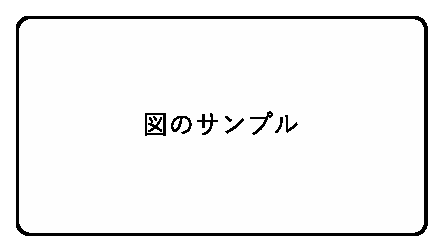
\includegraphics[scale=0.8]{sample-figure.eps}
 \caption{図のサンプル} \label{fig:sample}
\end{figure}
%

本文中で図を引用する場合は,図中で指定した\verb|label|を\verb|\ref|を用いて参照する.例えば上図で\verb|\label{fig:sample}|としている状態で本文中に``図\verb|\ref{fig:sample}|''と記述すると,texコンパイル後のファイルでは当該箇所が``図\ref{fig:sample}''に変換される.``図??''となる場合は,もう1度texコンパイルしてみて,それでも参照がされない場合は,ラベルが一致しているかどうか確認する.

% ----------------------------------------------------
\subsection{(第3レポートのみ)グループ内の役割分担}

第3レポートの対象となる回では,複数人のグループで作業を行うため,各回で誰が何を担当したのかも節(\verb|\subsection|)を用いて記載する.以下は記載例である.\texttt{tex}ソースに記載の通り,\verb|\description|環境を用いると良い.
%
\begin{description}
 \item[s123456 学生 なまえ] ネットワークの配線,環境の構築
 \item[s135791 相方 ひとりめ] プログラムのコーディング,デバッグ
 \item[s246802 相方 ふたりめ] コーディングのサポート
 \item[s369258 相方 さんにんめ] 3人の応援
\end{description}

% ----------------------------------------------------
\subsection{参考文献等}

書籍,インターネット上の情報などを参考にした場合,対象となるすべての回のものをまとめて,\verb|\thebibliography|環境を用いて出展を明記する.書き方は本ファイルの\texttt{tex}ソースを参考にする.
%
\end{comment}
%%%%%%%%%%%%%%%%%%%%%%%%%%%%%%%%%%%%%%%%%%%%%%%%%%%%%%%%%%%%%%%%%%%%%
% レポート作成の手引ここまで
%%%%%%%%%%%%%%%%%%%%%%%%%%%%%%%%%%%%%%%%%%%%%%%%%%%%%%%%%%%%%%%%%%%%%


%%%%%%%%%%%%%%%%%%%%%%%%%%%%%%%%%%%%%%%%%%%%%%%%%%%%%%%%%%%%%%%%%%%%%
% 第1回分(第1レポート内)サンプル
%   第1レポートでは,第1回~第4回分それぞれを 章 (\section) として1つのレポートにまとめること
%%%%%%%%%%%%%%%%%%%%%%%%%%%%%%%%%%%%%%%%%%%%%%%%%%%%%%%%%%%%%%%%%%%%%
%%% ------------------------------------------------------------------
%\newpage % ← 改ページ
\section{第1回 誤り制御符号(1):パリティ符号}

% ----------------------------------------------------
\subsection{実行結果}

%
% --- 実行結果ここから
\begin{lstlisting}[basicstyle=\ttfamily\footnotesize, frame=single]

********
  1ビット垂直パリティ検査を体験するプログラムです。
  7ビットの情報語に1ビットの検査語を加えて伝送します。
  ここでは偶数パリティを使用しています。
********

情報語を10進数で入力してください(0?127  エンターのみで終了): 入力値(10進数) = 12
入力値( 2進数) = 0001100

送信データ 0001100 0  (f6f5f4f3f2f1f0 p0)
受信データ 0001100 0  (f6f5f4f3f2f1f0 p0)
  算出された検査ビット = 0

伝送誤りはありません。

情報語を10進数で入力してください(0?127  エンターのみで終了): 入力値(10進数) = 12
入力値( 2進数) = 0001100

送信データ 0001100 0  (f6f5f4f3f2f1f0 p0)
受信データ 0000111 0  (f6f5f4f3f2f1f0 p0)
  算出された検査ビット = 1

伝送誤りが検出されました。

情報語を10進数で入力してください(0?127  エンターのみで終了): 入力値(10進数) = 12
入力値( 2進数) = 0001100

送信データ 0001100 0  (f6f5f4f3f2f1f0 p0)
受信データ 0001001 0  (f6f5f4f3f2f1f0 p0)
  算出された検査ビット = 0

伝送誤りはありません。

\end{lstlisting}
% --- 実行結果ここまで
%

\subsection{実行結果に対する考察}
%前節の実行結果より,~であることがわかる.また,~であるものと考えられる.
一回目の実行結果では、送信データと受信データは一致し、送受信が成功したことがわかる。\\
二回目の実行結果では、送信データと受信データは一致せず、送受信が失敗していたが、受信データには奇数個の1が含まれているため、伝送誤りを検出することができている。\\
三回目の実行結果では、伝送誤りが発生したが、1が偶数個含まれているので、受信側が伝送誤りを検出していない。これらの結果より、1ビット垂直パリティでは、伝送誤りを検出することはできるが、検出できない時もあることがわかった。


% ----------------------------------------------------
\subsection{課題} 

\kadai{今回の実験で作成したパリティ符号は,偶数パリティと奇数パリティのいずれであるかを答えよ.}

符号内の1の個数を偶数子に保つものであるため,偶数パリティである.

\kadai{1ビット水平パリティ符号について調査せよ.}

%1ビット水平パリティ符号とは,~~ものである.~~.
1ビット垂直パリティ符号はひとつの符号語の中の1の個数を数え、それに応じて0か1かが決定されるが、1ビット水平パリティ符号の場合はいくつかの符号語の中の同じnビット目の中に1がいくつあるか数え、それに応じて、nビット目が0か1かを決定した符号語を追加する方法である。

\kadai{1ビット水平パリティ符号と1ビット垂直パリティ符号を組み合わせることにより,1ビットの誤りを訂正できることを示せ.}

いくつかの符号語を送信し、1ビットの誤りが発生した時、各符号語の垂直パリティビットのうち、伝送誤りが検出されるものが必ず一つあり、水平パリティビットが集まった符号語の中にも伝送誤りが検出されるものが必ず一つある。垂直パリティビットの伝送誤りによりどの符号語で誤りが発生したのかがわかり、水平パリティビットの伝送誤りにより誤りが発生した符号語の中の何ビット目に誤りがあるのかがわかる。よって、1ビット水平パリティ符号と1ビット垂直パリティ符号を組み合わせることで1ビットの誤りを訂正することができる。
%
%%%%%%%%%%%%%%%%%%%%%%%%%%%%%%%%%%%%%%%%%%%%%%%%%%%%%%%%%%%%%%%%%%%%%
% 第1回分サンプルここまで
%%%%%%%%%%%%%%%%%%%%%%%%%%%%%%%%%%%%%%%%%%%%%%%%%%%%%%%%%%%%%%%%%%%%%

%%% ------------------------------------------------------------------
%\newpage
%\section{第x回 実験タイトル}

%....

%%% ------------------------------------------------------------------
%\newpage
%\section{第x回 実験タイトル}

%....

%%% ------------------------------------------------------------------
% --- 参考文献リストここから
%\newpage
\begin{thebibliography}{9}
%\bibitem{book-sample} 神崎映光,西川津ビビッド,出雲島猫,「書籍の参照はこんな感じ」,島大出版,1979年.
%\bibitem{url-sample} 島根大学 総合理工学部 数理・情報システム学科(情報系),http://www.cis.shimane-u.ac.jp/.
\bibitem{suihei-parity} ネットワークの基礎知識 誤り制御について , http://www5e.biglobe.ne.jp/~komichan/network/n1\_CRC.html
\end{thebibliography}
% --- 参考文献リストここまで
%

\end{document}
